\documentclass{article}
\usepackage{mathtools}
\usepackage{amsfonts}
\usepackage{amssymb}
\usepackage{tabu}
\usepackage{commath}
\usepackage{tikz}
\usetikzlibrary{decorations.pathreplacing}
\usepackage[section]{placeins}
\usepackage{nth}
\usepackage{xspace}
\usepackage[hidelinks]{hyperref}
\usepackage{defs}
\usepackage{fonts}

\newcommand{\main}{\texttt{main.cpp}\xspace}
\newcommand{\comm}{\texttt{comm.cpp}\xspace}
\newcommand{\utils}{\texttt{utils.cpp}\xspace}
\newcommand{\timer}{\texttt{timer.cpp}\xspace}
\newcommand{\inputdeck}{\texttt{input.deck}\xspace}
\newcommand{\kineticdeck}{\texttt{kinetic.deck}\xspace}
\newcommand{\floor}{\ensuremath{\mathtt{c\_floor}}\xspace}
\newcommand{\quadorder}{\ensuremath{\mathtt{quadOrder}}\xspace}
\newcommand{\dn}{\texttt{dn}\xspace}
\newcommand{\integer}{\texttt{int}\xspace}
\newcommand{\bool}{\texttt{bool}\xspace}
\newcommand{\float}{\texttt{float}\xspace}
\newcommand{\double}{\texttt{double}\xspace}
\newcommand{\chars}{\texttt{char[]}\xspace}
\newcommand{\N}{\ensuremath{\mathbb{N}}\xspace}
\newcommand{\Z}{\ensuremath{\mathbb{Z}}\xspace}
\newcommand{\Q}{\ensuremath{\mathbb{Q}}\xspace}
\newcommand{\R}{\ensuremath{\mathbb{R}}\xspace}
\newcommand{\C}{\ensuremath{\mathbb{C}}\xspace}
\newcommand{\assign}{\ensuremath{\mathrel{\texttt{:=}}}}
\DeclareMathOperator{\minmod}{minmod}
\DeclareMathOperator{\slopefit}{slopefit}
\DeclareMathOperator{\sgn}{sgn}
%\DeclareMathOperator*{\argmin}{arg\,min}
%\DeclareMathOperator*{\argmax}{arg\,max}

\newcommand{\integral}[1]{\ensuremath{\langle #1 \rangle}}
\newcommand{\closure}[1]{\ensuremath{\mathcal{E}(#1)}}
\newcommand{\twosphere}{\ensuremath{\mathbb{S}^2}\xspace}
\newcommand{\threespace}{\ensuremath{\mathbb{R}^3}\xspace}
\newcommand{\kinetic}{\texttt{kinetic}\xspace}
\newcommand{\moment}{\texttt{moment}\xspace}
\newcommand{\momopt}{\texttt{momopt}\xspace}

\frenchspacing
%\raggedright

\AtBeginDocument{\let\textlabel\label}

\title{\texttt{closures-2d} \\ Design Documentation}
\author{C. Kristopher Garrett, Tim Shaffer}

\begin{document}
\maketitle
\tableofcontents

\section{Purpose}
This software implements various numerical methods for
approximating the angular variable in kinetic transport in order
to study performance, accuracy, and robustness on common test problems.
Whereas fluid equations describe a vector of quantities dependent on space,
kinetic transport equations describe a scalar density of particles
depending on both space and velocity. Such numerical methods occur
frequently in production codes modeling certain physical systems, such as
neutron transport inside a reactor, neutrino transport in supernova simulations,
photon transport, and rarefied gas dynamics. Rather than simulating a
specific physical system, this software solves simpler problems that capture
issues commonly encountered in full simulations. Comparing the performance of
these numerical methods on our simplified problems can give researchers
insight into the behavior of similar methods in more complicated
implementations.

In addition to evaluating the methods themselves, this
software is written to allow study of
performance with modern high-performance computing resources. This software
optionally uses OpenMP and Message Passing Interface~(MPI) to carry
out parallel and concurrent computations. Studying the behavior of
numerical methods with such acceleration techniques provides reference for
implementations on large-scale problems.

This software also supports profiling measurements such as timings, flop rates,
memory rates, and cache misses. Using statistics about runtime performance,
we examined code optimizations, bottlenecks, etc. that occur
in our implementations.

\section{Problem}
This software simulates particles with unit speed that scatter isotropically according to a simple kinetic equation. 
The equation governing particle behavior takes the form
\begin{align}
    \label{eqn:kinetic}
    \partial_t f + \Omega \cdot \nabla_x f + \sigma_t f =
    \frac{\sigma_s}{4\pi} \integral{f}
\end{align}
where $f(x,\Omega,t)$ is the density of particles, $x \in \mathcal{D} \subset \mathbb{R}^2$ is position, $\Omega \in \twosphere \subset \threespace$ (the unit sphere)
is the direction of travel, $\sigma_t(x) \geq \sigma_s(x)$ are the total and scattering cross sections, and
\integral{\cdot} is shorthand for integration over \twosphere.
The boundary conditions implemented are either zero inflow boundary conditions or periodic boundary conditions depending on the initial condition discussed in Section~\ref{subsec:initcond}.

\subsection{Initial Conditions}
\label{subsec:initcond}
\FloatBarrier
The following initial conditions are implemented in this software.

\subsubsection{Gaussian Initial Condition}
\begin{figure}
    \centering
    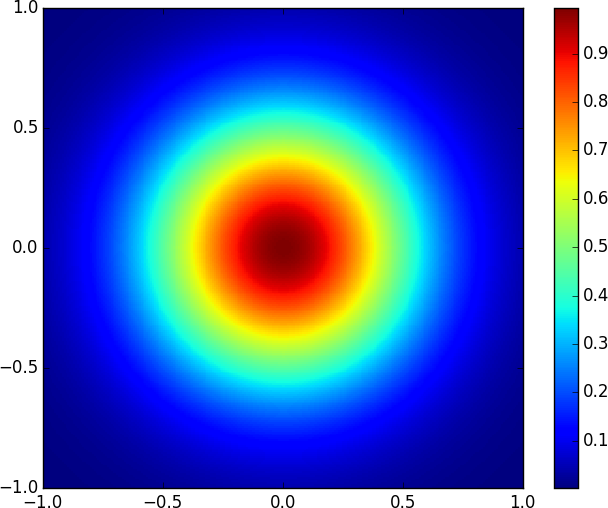
\includegraphics[height=0.3\textheight]{initcond_gaussian.png}
    \caption{Gaussian Initial Condition}
    \label{fig:gaussian_ic}
\end{figure}
In the Gaussian initial condition, a two dimensional Gaussian function
is placed with its peak at the center of the grid. Each point on the
initial grid is set to
\begin{equation}
    f(x,y,\Omega,t=0) = \max \left( \frac{1}{2 \pi \sigma_g^2} e^{-(x^2 + y^2) / (2 \sigma_g^2)}, \texttt{floor} \right), 
\end{equation}
where $\sigma_g$ is set by the user.
The cross sections $\sigma_s$ and $\sigma_t$ are constants defined by the user.
The zero inflow boundary condition is used.
Figure~\ref{fig:gaussian_ic} shows the initial condition of $\vint{f}$ for $\sigma_g = 0.4$. 

\subsubsection{Delta Initial Condition}
The limiting case, as $\sigma \to 0$, is the Delta initial condition.
This condition is meant to simulate an initial pulse of particles distributed
isotropically along an infinite line in space. The points on the initial grid
are initialized to
\begin{equation}
    f(x,y,\Omega,t=0) = \frac{1}{4\pi} \delta(x,y),
\end{equation}
approximating an infinitely narrow source at the origin. \comment{The source
doesn't have the $\frac{1}{4\pi}$ factor, is it introduced by scaling later?}
$\sigma_S$ and $\sigma_T$ are uniformly set to the configured
value for sigma.

\subsubsection{Lattice Initial Condition}
\begin{figure}
    \centering
    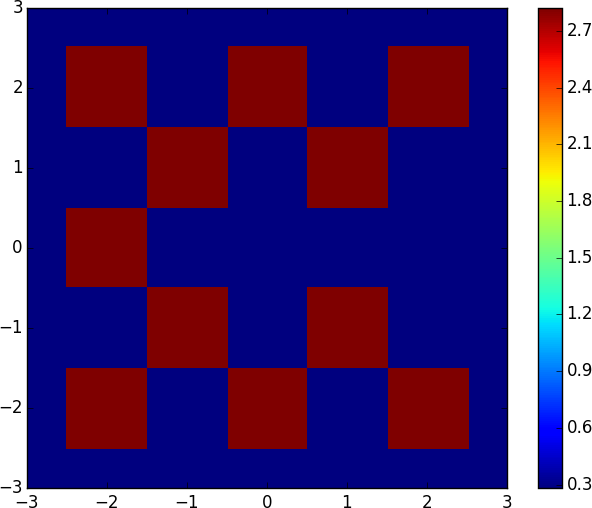
\includegraphics[height=0.3\textheight]{initcond_lattice-t.png}
    \caption{$\sigma_T$ for Lattice Initial Condition}
    \label{fig:lattice_ic}
\end{figure}
The Lattice initial condition corresponds to a checker board pattern
of highly scattering and highly absorbing regions~\cite{Brunner-Holloway-2005,Brunner-2002}.
This configuration is reminiscent of a
small section of a nuclear reactor core. The Lattice initial condition leaves the
grid initially empty, but has the most complicated scattering pattern of the initial
conditions. $\sigma_S$ and $\sigma_T$ are set to 1 at all positions, except
for several blocks arranged throughout the grid at which $\sigma_S=0$ and
$\sigma_T=10$.

\subsubsection{Smooth Initial Condition}
\begin{figure}
    \centering
    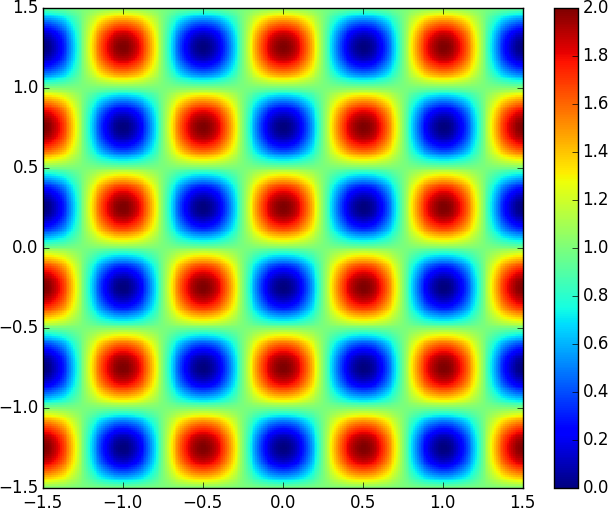
\includegraphics[height=0.3\textheight]{initcond_smooth.png}
    \caption{Smooth Initial Condition}
    \label{fig:smooth_ic}
\end{figure}
The Smooth initial condition is primarily intended for testing convergence.
This configuration initializes the grid points with a periodic boundary.
Each point in the initial grid is set to
\begin{align}
f(x,y,\Omega,t=0) = 1 + \sin(2\pi x)\cos(2\pi y).
\end{align}
$\sigma_S$ and $\sigma_T$ are uniformly set to the configured
value for sigma.


\section{Angular Approximations}
\subsection{Discrete Ordinates}
The \kinetic solver is an implementation of the discrete ordinates method, also known
as $\mathrm{S}_N$.
Our implementation uses a Chebyshev-Legendre quadrature on the unit sphere.
A Lebedev quadrature is also implemented for this solver,
but is considered experimental.
Details of the quadratures are given in Section~\ref{subsec:quadratures}. Let
$\{\Omega_1, \dots, \Omega_Q\} \in \twosphere$ be be a set of nodes with
corresponding weights $\{w_1, \dots, w_Q\}$. Then from Equation~\ref{eqn:kinetic}
\begin{equation}
    \partial_t f_q + \Omega_q \cdot \nabla_x f_q + \sigma_t f_q=
    \frac{\sigma_s}{4\pi} \sum_{q'=1}^Q w_{q'} f_{q'},
\end{equation}
where $f_q(x,t) \approx f(x, \Omega_q, t)$ for $q = 1, \dots, Q$.

This implementation uses Heun's method to achieve second order convergence. Edge values
are computed via upwinding. For approximate slopes, the double minmod limiter is used.

\subsection{Moment Solvers}
\comment{Show basic setup. Then define $\mathcal{E}(\bu)$ for each type.}
The \moment solver uses standard spectral methods with Equation~\ref{eqn:kinetic}. The real
spherical harmonics serve as an orthonormal basis of $L^2$ with respect to
\twosphere for the expansion of the moments. Let
$\mathbf{m}(\Omega) =
(Y_{0,0}, Y_{1,-1}, Y_{1,0}, Y_{1,1}, \dots, Y_{N,-N}, \dots, Y_{N,N})^T$
be a vector of spherical harmonics up to and including degree $N$. The moments
with respect to $\mathbf{m}$ are given by
\begin{equation}
    \mathbf{u}^{\textrm{exact}}(\mathbf{x}, t) =
    \integral{\mathbf{m}(\Omega) f(\mathbf{x}, \Omega, t)}
\end{equation}
since $u_{\ell,m} = f_{\ell,m}$ and the collision operator is diagonalized.
\comment{Separate exact u from approximate u.}
The exact moment system is given by
\begin{equation}
    \partial_t \mathbf{u} + \nabla_x \cdot \integral{\Omega\mathbf{m}f} =
    \Dif \mathbf{u},
\end{equation}
but this formulation is not closed. Thus $f$ is replaced with a $\mathrm{P}_N$
moment closure $\closure{\mathbf{u}}$ such that
$\integral{\mathbf{m}\closure{\mathbf{u}}} = \mathbf{u}$. In this case,
\begin{equation}
    \closure{\mathbf{u}} = \sum_k u_k m_k = \mathbf{u}^T \mathbf{m}
\end{equation}
yielding the closed moment system
\begin{equation}
    \partial_t \mathbf{u} + \nabla_x \cdot
    \integral{\Omega\mathbf{m}\closure{\mathbf{u}}} = \Dif \mathbf{u}.
\end{equation}
It is only necessary to use the spherical harmonics $Y_{\ell,m}$ such that
$\ell + m$ is even. \comment{State why...}



\subsubsection{Entropy Minimization}
Suppose $\closure{\bu}$ is obtained as an entropy minimization
\begin{equation}
    \label{eqn:entropy}
    \mathcal{E}(\mathbf{u}) = \argmin_{g \in L^1} \integral{\eta(g)} \quad
    \textnormal{subject to} \quad \integral{\mathbf{m}g} = \mathbf{u}
\end{equation}
\comment{Fill in the rest here.}



\subsubsection{P$_N$}
$\closure{\bu} = \bm^T \bu$.
Can get this by (1) truncating, (2) least squares, (3) minimizing entropy.
\comment{Fill in a little bit.}

Various filters can also be applied to suppress oscillations in spherical harmonics.

\begin{itemize}
    \item The Hauck filter is described in \cite{Hauck-McClarren-2010}.
    Let $N$ be the moment order and $\omega$ be the filter tune, and define
    \begin{equation}
        \alpha = \frac{\omega}{N^2 (\sigma_T L + N)^2}.
    \end{equation}
    Scale each moment by
    \begin{equation}
        \frac{1}{1 + \alpha n^2 (n+1)^2}
    \end{equation}
    for the $n$\textsuperscript{th} moment.

    \item The Spline filter is given in \cite{Radice-2013}.
    With moment order $N$ and filter tune $\sigma_e$, let
    \begin{equation}
        s = \frac{-\sigma_e \Delta t}{\log F(N/(N+1))}
    \end{equation}
    where $F(x) = 1/(1 + x^4)$. The scale factor is given by
    \begin{equation}
        F(n/(N+1))^s.
    \end{equation}

    \item The Lanczos filter is taken from~\cite{Radice-2013}.
    Again with moment order $N$ and filter tune $\sigma_e$, let
    \begin{equation}
        s = \frac{-\sigma_e \Delta t}{\log L(N / (N+1))}
    \end{equation}
    where
    \begin{equation}
        L(x) = \begin{dcases*}
            1 & when $x=0$ \\
            \frac{\sin x}{x} & otherwise.
        \end{dcases*}
    \end{equation}
    Now the moment scale factor is
    \begin{equation}
        L(n / (N+1))^s.
    \end{equation}
\end{itemize}

\subsection{M$_N$ and PP$_N$}
One serious drawback of the P$_N$ method is the possibility of non-realizable
solutions with negative densities, oscillatory approximations of nonsmooth
solutions. 
\comment{Can just put the definitions for $\eta$ and other stuff here for M$_N$ and PP$_N$.}

Nonlinear approaches can ensure positivity,
but come with increased complexity and computational cost. In general,
entropy-based moment closures, like the \momopt solver, can be cast in the
framework of the following minimization problem
\begin{equation}
    \label{eqn:entropy}
    \mathcal{E}(\mathbf{u}) = \argmin_{g \in L^1} \integral{\eta(g)} \quad
    \textnormal{subject to} \quad \integral{\mathbf{m}g} = \mathbf{u}
\end{equation}
where $\eta$ is a smooth, strictly convex, coercive\footnote{We define a
function $\eta$ to be coercive if
$\lim_{r \to \infty} \frac{\eta(r)}{|r|} = \infty$} function. For the
\momopt solver, $\eta(\mathbf{r}) = \mathbf{r} \log \mathbf{r} - \mathbf{r}$
and its Legendre dual\footnote{The Legendre dual of $\eta$ is given by
$\eta_*(s) = rs - \eta(r)$ where $s = \eta'(r)$. By differentiating this
relation, one can show that $r = \eta'_*(s)$. Thus $\eta'$ and $\eta'_*$ are
inverses of each other.} $\eta*(\mathbf{s}) = \mathbf{e^s}$.

The solution to Equation~\ref{eqn:entropy}, if it exists, is given by
\begin{equation}
    \mathcal{E}(\mathbf{u}) = \eta'_*(\hat{\mathbf{\alpha}}(\mathbf{u})^T \mathbf{m})
\end{equation}
where $\eta_*$ is the Legendre dual of $\eta$ and $\hat{\mathbf{\alpha}}(\mathbf{u})$
solves the dual problem
\begin{equation}
    \hat{\mathbf{\alpha}}(\mathbf{u}) = \argmin_{\mathbf{\alpha} \in \R^n}
    \left\{ \integral{\eta_*(\mathbf{\alpha}^T\mathbf{m})} -
    \mathbf{\alpha}^T \mathbf{u} \right\}.
\end{equation}

\section{Implementation}
\subsection{Quadratures}
\label{subsec:quadratures}
\comment{Let's go over this.  Some of the wording is not quite right.}
The Chebyshev-Legendre quadrature \cite{atkinson-1982} is used for numerical integration over
\twosphere in all of the solvers. This quadrature is constructed from an
$n$ point Gauss-Legendre rule, which exactly integrates smooth functions of
order less than $2n-1$. Since this is a 2D code, it is only necessary
to integrate over the upper half of \twosphere, which is divided into
$n$~layers along the $z$ axis. Abscissae and weights from GSL are arranged
in a circle around \twosphere at each layer, giving $n^2$ points on the
upper half of \twosphere. The Chebyshev-Legendre quadrature is not optimal
with respect to number of points, but is simple to implement. The Lebedev
quadrature, for example, is optimal in number of points, and an experimental
implementation is available for the \kinetic solver. This quadrature, however,
uses a more complicated arrangement of points, making exploiting symmetries
in the integral more difficult. In addition, the points of the
Chebyshev-Legendre quadrature are simply the Cartesian product of $n$ angles
spaced around a circle and $n$ values of $z$. This structure could allow the
evaluation of integrals via the Chebyshev-Legendre quadrature to be optimized
more easily than the Lebedev quadrature, which is arranged nontrivially and
becomes denser with increasing order.

The fixed-order
Gauss-Legendre integration points and weights from GSL will be referred to as $\mu_i$,
and $w_i$, respectively. Next, the
azimuthal angles of quadrature, $\phi_k$, are calculated as
\begin{equation}
    \phi_k = \frac{(k + 0.5)\pi}{Q}
\end{equation}
for $k \in \Z$ and quadrature order $Q$ such that $0 \leq k < 2Q$,
placing $2Q$ points evenly around the unit circle, and
the points are mapped into cylindrical coordinates $\xi_i,\eta_i$.

For $q_1,q_2$ such that $0 \leq q_1 < Q / 2$ and
$0 \leq q_2 < 2Q$, let
$i = 2q_1Q + q_2$. Now 
\begin{align}
    W_i &= \frac{2\pi w_{q_1}}Q \\
    \xi_i &= \sqrt{1 - \mu_{q_1}^2} \cos \phi_{q_2} \\
    \eta_i &= \sqrt{1 - \mu_{q_1}^2} \sin \phi_{q_2}.
\end{align}

Once the quadrature points and weights are computed, each integral over \twosphere
can be calculated as
\begin{equation}
    \int_{\twosphere} f(x,y,\Omega,t) \dif \Omega = \sum _{i=1}^Q W_i f(x,y,\omega_i,t)
\end{equation}
where $\omega_i$ is the direction $(\xi_i,\eta_i)$.

\subsection{Flux Calculations}
\comment{Is this worth including/expanding?}
All the solvers compute flux by examining values of neighboring cells in the
$x$ and $y$ directions.  The exact operations vary with each solver.

\subsection{Time}
Time steps are carried out via Heun's method which is an explicit two-stage Runge-Kutta method that is second order accurate. 
If $f(x,y,\Omega,t)$ is the density a a given position, direction, and time,
then we apply two time steps in succession to obtain a first approximation
$\tilde{f}(x,y,\Omega,t+2\Delta t)$. Now the calculated time step is
the average of the approximation and the starting value, that is
\begin{equation}
f(x,y,\Omega,t+\Delta t) = \frac{1}{2}\left(
        f(x,y,\Omega,t) + \tilde{f}(x,y,\Omega,t+2\Delta t)
    \right).
\end{equation}
Notice Heun's method is the average of two Euler steps which puts it into the category of a strong stability preserving (SSP) method.
SSP methods preserve properties satisfied by the Euler method.
In particular, the software uses this method to ensure positivity for some methods.

\subsection{Space}
\comment{All the implementation stuff should be here.  Not in the appendix.  Add proof of positivity for S$_N$ and M$_N$ and PP$_N$.}
Space is discretized using the finite volume method. The problem domain is
decomposed into a regular grid of cells with an additional halo of ghost cells
to enforce the boundary condition and allow synchronization with other nodes.
At each update, the program first computes the flux at each cell, then updates
the cell values according to the kinetic transport equation. Several of the
solvers guarantee positivity on the grid.

\comment{The minmod preserves positivity.  Need to show this.}
Some of the solvers employ a double minmod slope limiter to reduce oscillations
introduced by the spatial scheme. This function is defined as
\begin{equation}
    \minmod (x, y) = \sgn'(x) \max\left(0, \min\left(|x|, y \sgn'(x)\right)\right)
\end{equation}
where
\begin{equation}
    \sgn'(x) =
    \begin{dcases*}
        1  & if $x \geq 0$ \\
        -1 & if $x < 0$.
    \end{dcases*}
\end{equation}
In particular, note that $\minmod (x,y)$ is
\begin{itemize}
    \item 0 if $xy < 1$
    \item $\min\{x, y\}$ if $x,y > 0$
    \item $-\min\{|x|, |y|\}$ if $x,y < 0$.
\end{itemize}

For the \kinetic solver (implementing $S_N$), the timestep
$\Delta t$ is chosen with respect to the cell size so as not to violate
the CFL condition:
\begin{equation}
    \Delta t = \frac{c \Delta x \Delta y}{2(\Delta x + \Delta y)}.
\end{equation}
where $c$ is the configured CFL factor.
To eliminate the possibility of negative density due
to scattering, an additional term is included in the CFL check.
\comment{Is this implemented, or did we just talk about it?}

The \momopt solver also ensures positivity as part of the flux calculations.
The flux is based on an ansatz grid with strictly positive values. For $M_N$,
the ansatz grid value $a$ at each cell and direction is given by
\begin{equation}
    a = \exp (\alpha^T m).
\end{equation}
For $PP_N$,
\begin{equation}
a =
\begin{dcases}
    \frac{1}{2}k + \frac{1}{2}\sqrt{k^2 + 4\delta} & \text{if } k > 0 \\
    \frac{-\delta}{\frac{1}{2}k - \frac{1}{2}\sqrt{k^2 + 4\delta}} & \text{if } k \leq 0
\end{dcases}
\end{equation}
where $k = \alpha^T m$.

\subsection{Optimization Procedure}
\dots

\section{Program Layout}
\comment{Make this nicer.  Introduce each solver here (i.e. kinetic\_solver) as associated with for instance S$_N$.}
\comment{Describe binary file formats.}
All options controlling the runtime operation of the program reside in
\texttt{input.deck}. Comments prefixed with \texttt{\#} are allowed,
and options not used by the selected solver are ignored. Available options are
listed in Section~\ref{sec:options}, and example options for the various
solvers are included in the \texttt{examples/} directory.
The outputs are binary files with
extensions \texttt{.sn}, \texttt{.pn}, and \texttt{.opt}, depending on
the solver. Python code for reading and working with these files is provided
in \texttt{util/formats.py}.

The common functionality is split up among the files in \texttt{src/}.
\begin{itemize}
 \item \texttt{main.cpp} -- Entry point of program
 \item \texttt{comm.cpp} -- Controls MPI communication
 \item \texttt{utils.cpp} -- Helper functions used throughout the code
 \end{itemize}
The solver code has an approximately common layout, e.g. in \texttt{src/moment/}
\begin{itemize}
 \item \texttt{moment\_init.cpp} -- Read config, set up quadrature and filters, etc.
 \item \texttt{moment\_boundaries.cpp} -- Communicate boundary data with other nodes
 \item \texttt{moment\_update.cpp} -- Solve flux, update the grid with time, etc.
 \item \texttt{moment\_output.cpp} -- Write out results
\end{itemize}

When using MPI, \comm communicates boundary data between nodes.
\texttt{Solver::getInnerBoundaries} is first called to obtain grid data on the
boundaries of the current node's region of the domain. Next, each node trades boundary
data with its neighbors to the north, south, east, then west via
\texttt{MPI\_ISend} and \texttt{MPI\_IRecv}. Finally, the node calls \texttt{Solver::setOuterBoundaries}
to update its grid with the data from neighboring nodes.
\comment{Note scaling has not been tested for MPI.}

\section{Results}
\dots


\bibliographystyle{plain}
{\footnotesize
\bibliography{refs}}

\end{document}
